\documentclass[a4paper, 12pt]{article}
\usepackage{listings} 
\usepackage{xcolor}
\usepackage{mdframed}
\usepackage{graphicx}
\definecolor{code-gray}{gray}{0.93}

\begin{document}
\title{ECE 341 - Lab \#1}
\author{Collin Heist}
\date{\today}
\maketitle
\pagenumbering{roman}
\tableofcontents
\lstlistoflistings
\newpage
\pagenumbering{arabic}

\section{Introduction}
The goal of this lab is to familiarize ourselves with the basics of I/O on this development board. My preliminary idea of using bit-masking to ignore non-essential bits of \textbf{PORTG}, and then encode which LED to light up using a 'one-hot' number worked exactly as planned.

Before beginning the lab, I did read about the various \textbf{SFRs} available on this micro-controller that allow for more convenient use of the I/O pins. Although, for this specific implementation I did not use many SFR's, and instead opted to use the Peripheral-provided functions (thanks to their convenience).

\section{Implementation}
To begin, I read the already prepared function names and descriptions to understand what each function needs to do. Afterwards, I started with the \textbf{initialize\_system()} function, and added the code shown in Listing 1.

	\begin{mdframed}[backgroundcolor=code-gray, roundcorner=10pt,
								innerleftmargin=5, innertopmargin=5, innerbottommargin=5]	
	\begin{lstlisting}[language=C, caption=I/O Pin Initialization, tabsize=2]
	void initialize_system() {
		Cerebot_mx7cK_setup();

		PORTSetPinsDigitalIn(IOPORT_G, BTN1 | BTN2);
		PORTSetPinsDigitalOut(IOPORT_G, LED1 | LED2 |
			LED3 | LED4);
		PORTClearBits(IOPORT_G, LED1 | LED2 |
			LED3 | LED4);
	}
	\end{lstlisting}
	\end{mdframed}
	
This code comes directly after the hardware initialization, and my addition of those \textbf{PORT...} function calls simply configures \textbf{PORTG} in specific ways. In particular, the pin locations associated with button 1 and 2 are configured as inputs, while the locations of LED's 1 through 4 are configured as outputs. To be certain the LED's start as \textit{off}, that final function call sets those bit positions to 0.
\newpage

The next function I changed was \textbf{read\_buttons()}. My final function is shown below, in Listing 2.

	\begin{mdframed}[backgroundcolor=code-gray, roundcorner=10pt,
								innerleftmargin=5, innertopmargin=5, innerbottommargin=5]	
	\begin{lstlisting}[language=C, caption=Button Reading, tabsize=2]
	int read_buttons(void) {
		return (PORTG & (BTN1 | BTN2));
	}
	\end{lstlisting}
	\end{mdframed}
	
The above code reads from the \textbf{PORTG} register and ignores the non-essential bits (hence the bit-mask for \textbf{BTN1} and \textbf{BTN2}). This new value is simply whether or not both buttons are pressed. It is calculated and returned as an integer. Because of the bit masking, and due to the fact that no shifting nor parsing occurs in this function, the value is a binary number with 1's or 0's in either the 6th or 7th position.

My changes for the \textbf{decode\_buttons()} function are shown in Listing 3.

	\begin{mdframed}[backgroundcolor=code-gray, roundcorner=10pt,
								innerleftmargin=5, innertopmargin=5, innerbottommargin=5]	
	\begin{lstlisting}[language=C, caption=Button Decoding, tabsize=2]
	int decode_buttons(int buttons) {
		int status = (buttons & (BTN1 | BTN2)) >> 6;

		return (1 << status);
	}
	\end{lstlisting}
	\end{mdframed}

Despite being such a small section of code, this function actually does quite a bit. Using the passed \textit{buttons} integer, who's bits correspond to whether Button 1 or 2 is pressed, the first line ignores the non-button bits (even though they should be zero already due to \textbf{read\_buttons()}) and then shifts them over so that \textbf{BTN1} is in bit position 0. This value, \textbf{status}, is then used to \textit{left-shift} a binary 1 over that many places. That value is then returned, and is equivalent to a one-hot encoded number where bit positions 0-3 represent which LED to light up.

The final function I changed was the \textbf{control\_leds()} function, which takes a provided integer and in turn lights up the appropriate LED's on the board. My code is shown in Listing 4.
\newpage

	\begin{mdframed}[backgroundcolor=code-gray, roundcorner=10pt,
								innerleftmargin=5, innertopmargin=5, innerbottommargin=5]	
	\begin{lstlisting}[language=C, caption=Controlling the LED's, tabsize=2]
	void control_leds(int leds) {
		switch (leds) {
			case 1:
				PORTSetBits(IOPORT_G, LED1);
				PORTClearBits(IOPORT_G, LED2 | LED3 | LED4);
				return;
			case 2:
				PORTSetBits(IOPORT_G, LED2);
				PORTClearBits(IOPORT_G, LED1 | LED3 | LED4);
				return;
			case 4:
				PORTSetBits(IOPORT_G, LED3);
				PORTClearBits(IOPORT_G, LED1 | LED2 | LED4);
				return;
			case 8:
				PORTSetBits(IOPORT_G, LED4);
				PORTClearBits(IOPORT_G, LED1 | LED2 | LED3);
				return;
		}
	}
	\end{lstlisting}
	\end{mdframed}
	
I wrote this function to take a one-hot encoded four-bit number (like that returned by \textbf{decode\_buttons()}) and light the appropriate LED, based off which bit is 'hot.' I implemented this quite plainly with a switch-case statement that has a condition for each of the possible LED's to light up. The values used (1, 2, 4, and 8) all correspond to one bit in the \textbf{leds} variable. The final step is to clear the non-lit LED's so that they do not stay on forever.

After all of this, the only thing left was to implement these functions into the infinite loop of the micro-controller. This was by the most simple part, and is shown below:\newpage

	\begin{mdframed}[backgroundcolor=code-gray, roundcorner=10pt,
								innerleftmargin=5, innertopmargin=5, innerbottommargin=5]	
	\begin{lstlisting}[language=C, caption=Main Infinite Loop, tabsize=2]
	int main() {
		initialize_system();
		while (1) {
			int buttons = read_buttons();	
			int leds    = decode_buttons(buttons);
			control_leds(leds);
		}
		return 1;
	}
	\end{lstlisting}
	\end{mdframed}

This code simply implements the function I described above. After initializing the board and setting the appropriate pins as outputs / inputs, an infinite loop reads the buttons, decodes them, and then updates the LED's.

\section{Testing and Validation}
The only test necessary to verify that my above code worked as expected was to test each combination of buttons, and verify that the LED's lit up appropriately. I accomplished this by pressing \textbf{BTN1} and \textbf{BTN2} in all four combinations (including neither being pressed) and all of the LED's lit up as expected.

Luckily, I had no need for debugging instrumentation during this lab. The only 'debugging' necessary was the visual observation of whether the LED's illuminated correctly or not. And, as described in the lab, that's somewhat the point of this kind of exercise. The addition of code to control an LED is very simple and can produce a very clear and direct indication of whether code is working or not.

If you wanted to manually verify whether my project works, all you'd need to do is open the project in \textbf{MPLAB X}, make sure the board is on and connected, and then run it from within the IDE. Once it is running (the play button should be grayed out), simply observe each of the LED's on the board. The following table shows under what conditions they should be illuminated (where 1's are ON / pressed, and 0's are OFF / not pressed). By pressing all four button combinations, the code can be verified manually.
\newpage

\begin{table}
\centering
\begin{tabular}{c|c|c|c|c|c}
\textbf{BTN2} & \textbf{BTN1} & \textbf{LED4} & \textbf{LED3} & \textbf{LED2} & \textbf{LED1} \\
\hline
0 & 0 & 0 & 0 & 0 & \textbf{1} \\
0 & \textbf{1} & 0 & 0 & \textbf{1} & 0 \\
\textbf{1} & 0 & 0 & \textbf{1} & 0 & 1 \\
\textbf{1} & \textbf{1} & \textbf{1} & 0 & 0 & 0 \\
\end{tabular}
\end{table}

\section{Questions}
\begin{enumerate}
\item There are many different ways to read from and write to a specific I/O pin on the processor. Given that we have access to the Peripheral Libraries provided in \textbf{MPLAB X}, the available macros for each pin make these types of tasks very easy. To write to a specific pin without affecting others, the general premise is to use \textit{bit-masks}. There are ones provided by the Peripheral Libraries that correspond to individual bit positions (i.e. \textbf{BIT\_0}, \textbf{BIT\_15}, etc.) but even without the nicely defined ones, custom made bit-masks allow writing to the I/O pin a register at a time (as must be done) without modifying any pins that you do not want changed. Reading from the pins is easier, as you do not have to worry about affecting other pins on the same register, so simply using a bit mask to ignore other pins is often suffice.

\begin{figure}[h]
\centering
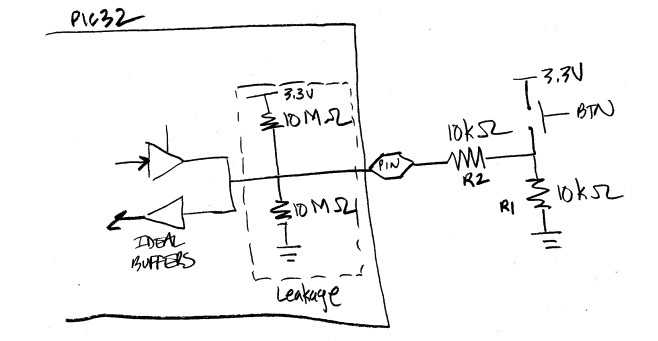
\includegraphics[width=1\textwidth]{Schematic}
\caption{Abstraction of the PIC32 I/O cell}
\end{figure}

\newpage
\item To derive the equation for the voltage at the I/O pin and the current through $R_2$, if the button is \textit{not} pressed, I used the following KVL:
$$\frac{3.3-V_{pin}}{R_{big}}=\frac{V_{pin}}{R_{big}}+\frac{V_{pin}}{R_2+R_1}$$
After solving for \textit{$V_{pin}$} and the current through $R_2$...
\begin{equation}V_{pin}=\frac{1.65*(R_1+R_2)}{R_1+R_2+0.5*R_{big}}\end{equation}
\begin{equation}I_{R_2}=\frac{V_{pin}}{R_2+R_1}\end{equation}

And if the button \textit{is} pressed, the following KVL applies:
$$\frac{3.3-V_{pin}}{R_{big}}+\frac{3.3-V_{pin}}{R_2}=\frac{V_{pin}}{R_{big}}$$
Once again, solving for \textit{$V_{pin}$}...
\begin{equation}V_{pin}=\frac{1.65*(R_2+R_{big})}{R_2+0.5*R_{big}}\end{equation}
\begin{equation}I_{R_2}=\frac{3.3-V_{pin}}{R_2}\end{equation}
Using actual values, it's shown that when the button is not pressed, $V_{pin}=6.574 mV$, $I_{R_2}=0.3287 \mu A$. And when the button is pressed, $V_{pin}=3.29671 V$ and $I_{R_2}=0.329 \mu A$

\item The purpose of the external pull-down resistor ($R_1$ in the diagram) is to bring the voltage on the Pin near ground when the button is disconnected (not pressed). This prevents the voltage at the pin from "floating" and and possibly damaging the pin or accidentally being read as a High (1). In our provided figure, if $R_1$ were removed, there would be no current through $R_2$ when the button was not pressed. This results in our internal circuitry essentially becoming a voltage divider, leading to the voltage at the pin becoming 1.65 V, which is a dangerous zone to be in for I/O pin. This is because 1.65 V falls exactly between the logical \textit{high} and \textit{low}, and natural variance might lead to an inconsistent or unstable reading on that pin.

\item According to the \textbf{Cerebot 32MX7cK} schematic, there is an internal 470 $\Omega$ resistor between the LED and ground. After the 0.7 V drop, that means there is 5.543 mA of current through the pin. The board's reference manual says that the micro-controller can source or sink at most 18 mA on any individual pin, and a total of 200 mA across all the I/O pins available.
\end{enumerate}

\section{Conclusion}
This lab was far more insightful than Lab \#0. Interacting with the micro-controller and using its peripherals to interface with me (the user) was very interesting and useful than running generic C-code. Although, once again I cannot think of any limitations highlighted by this lab. The only thing that comes to mind is how 'limiting' it could be to have to initialize all the appropriate pins as input or output before the code has run, and if you do it incorrectly then the IDE has no warning system. I understand why that is the case, but it could be problematic nonetheless.

\end{document}